% Imports
\documentclass[journal]{IEEEtran}
\usepackage[spanish]{babel}
\usepackage[utf8]{inputenc}
\usepackage{graphicx}
\usepackage{hyperref}
\usepackage{amsmath}
\usepackage{amssymb}
\usepackage{multirow}

% Documento
\begin{document}
\title{Estimación de la probabilidad condicional de ganar un punto en tenis profesional}
\author{Federico Soler}
\maketitle

\begin{abstract}
Analizar un encuentro competitivo permite examinar cómo las decisiones de los jugadores modifican su desarrollo. En ajedrez, plataformas como \textit{Chess.com} facilitan este análisis mediante una barra que representa la ventaja posicional estimada por un motor y se actualiza después de cada movimiento. Este trabajo explora si ese principio de evaluación secuencial puede trasladarse al tenis profesional, utilizando la probabilidad condicional de ganar el punto como medida del balance entre ambos jugadores después de cada tiro.

Para ello, se entrena un ensamble supervisado de \textit{XGBoost} sobre registros del \textit{Match Charting Project}, utilizando características dinámicas del intercambio y una ventana temporal del tiro actual y los dos anteriores ($t,t-1,t-2$). El modelo alcanzó un desempeño comparable al de investigaciones previas, con un Accuracy del \textbf{60.51\%}, un AUC-ROC de \textbf{0.6410}, un \textit{Brier Score} de \textbf{0.2292}, una \textit{Log Loss} de \textbf{0.6484}, un \textit{Expected Calibration Error} de \textbf{0.48\%}, un Kappa de Cohen de \textbf{0.1656} y $F_1$-scores de \textbf{68.83\%} para el sacador y \textbf{46.15\%} para el restador. Los resultados confirman que las secuencias recientes de golpes contienen señal suficiente para rastrear, tras cada tiro, la evolución de la ventaja del sacador sin recurrir al ranking, al marcador ni a la identidad de los jugadores.
\end{abstract}

\section{Introducción}
En el ajedrez, el análisis de partidas se apoya ampliamente en la barra de evaluación ofrecida por plataformas como \textit{Chess.com} \cite{chesscom2026, chesscom_evaluation}, la cual se ajusta dinámicamente tras cada jugada para reflejar qué bando tiene la iniciativa. Calculada mediante motores como \textit{Stockfish} \cite{stockfish2026, stockfish_evaluation}, esta herramienta permite comprender de forma inmediata el impacto de cada decisión sobre las perspectivas del juego \cite{Regan2011IntrinsicChess}. Desarrollar una perspectiva similar en el tenis profesional plantea el desafío de modelar el peloteo no como un resultado cerrado, sino como una secuencia de golpes donde cada tiro modifica la probabilidad condicional de ganar el punto.

En las transmisiones y análisis de tenis, predominan tradicionalmente las estadísticas acumuladas (aces, primeros saques, tiros ganadores y errores no forzados). Si bien estas cifras describen el volumen global del juego, resultan insuficientes para comprender el desarrollo táctico del intercambio. Formalmente cada punto vale lo mismo según las reglas \cite{usta2023tennis}, pero la ventaja se construye y disputa impacto tras impacto. En este sentido, la literatura fundamenta la importancia del modelado tiro a tiro \cite{Floyd2020ShotByShot} para dimensionar objetivamente el peso de cada decisión en el peloteo.

En el ámbito del tenis, la literatura científica ha transitado desde el análisis notacional tradicional \cite{o2001notational} y las taxonomías de golpes \cite{kovalchik2018shot} hacia marcos analíticos orientados a medir el balance del juego. Diversos estudios formalizaron índices de ventaja posicional y coordinación interpersonal \cite{carvalho2013elucidating, vanMeurs2021PositionalAdvantage}, examinaron la dinámica espaciotemporal del peloteo \cite{emery2020augmenting}, modelaron fluctuaciones de \textit{momentum} \cite{liu2025quantifying} y exploraron plataformas comerciales de la industria \cite{infosysAtp2026}. En el plano probabilístico, los antecedentes abarcan formulaciones estocásticas \cite{floyd2017applying}, modelos jerárquicos bayesianos \cite{ingram2019point}, minería de patrones tácticos \cite{liu2023insight} y algoritmos de aprendizaje automático para pronóstico de partidos \cite{kovalchik2016searching, rui2024forecasting, poudel2026unified, illum2025analysis}. No obstante, investigaciones recientes advierten que muchos modelos agregados sufren severas fugas de datos (\textit{data leakage}) al incorporar variables acumuladas durante o después del partido \cite{gao2021random}. Frente a estas limitaciones, el \textit{Match Charting Project} (MCP) \cite{sackmann2026mcp} surgió como un repositorio público con registros estructurados golpe por golpe, posibilitando la exploración de modelos predictivos abiertos basados en gradiente potenciado \cite{youtubeXGBoostTennis2025}.

Por su parte, el ajedrez computacional resolvió tempranamente la evaluación de posiciones intermedias combinando algoritmos de búsqueda con poda alfa-beta \cite{knuth1975analysis} y, más recientemente, funciones de evaluación neurales eficientemente actualizables (NNUE) \cite{nasu2018nnue, Klein2022NeuralNF, stockfish_nnue}, capaces de detectar quiebres decisivos de ventaja incluso en secuencias tácticas breves \cite{hooper1992oxford}. Para trasladar una capacidad análoga a la naturaleza tabular y heterogénea del MCP, la literatura metodológica demuestra que los árboles de decisión CART \cite{breiman1984classification} y los ensambles de gradiente potenciado (\textit{boosting}) \cite{hastie2009elements} han mostrado resultados competitivos frente a arquitecturas neuronales profundas en diversas tareas con datos tabulares \cite{grinsztajn2022tree}. Esto fundamenta la elección de algoritmos como \textit{XGBoost} \cite{chen2016xgboost} optimizados computacionalmente \cite{mitchell2017xgboostgpu}. Para auditar rigurosamente estos modelos sin incurrir en fugas de información \cite{kaufman2012leakage}, la literatura describe alternativas para la selección de hiperparámetros \cite{bergstra2012random}, la interpretación de variables mediante valores SHAP \cite{lundberg2017unified} y una evaluación que combine métricas de discriminación y concordancia (AUC-ROC \cite{fawcett2006introduction, hanley1982meaning}, Kappa \cite{cohen1960coefficient}) con evaluación de pérdida logística (\textit{Log Loss} \cite{good1952rational, bishop2006pattern}) y técnicas de calibración probabilística empírica \cite{brier1950verification, platt1999probabilistic, zadrozny2002transforming, guo2017calibration}.

Este trabajo propone estimar tiro a tiro la probabilidad condicional de que el jugador al servicio termine ganando el punto a partir de las características observables del intercambio en una ventana temporal tripartita ($t, t-1, t-2$), prescindiendo deliberadamente de la identidad de los jugadores, de sus rankings, del marcador del partido, del torneo y de la superficie. La utilidad práctica de este modelado se ilustra analizando un punto de la final del US Open 2009 entre Roger Federer y Juan Martín del Potro, examinando cómo evoluciona la probabilidad del tanto a lo largo de un intercambio real.

El artículo se organiza de modo que la Sección II aborda el marco teórico, la Sección III detalla la ingeniería de características y la arquitectura del modelo, la Sección IV expone los resultados y el caso de estudio, y la Sección V presenta la conclusión.

\begin{figure*}[htpb]
    \centering
    \includegraphics[width=0.19\textwidth]{01. Tablero Inicializado.png}
    \hfill
    \includegraphics[width=0.19\textwidth]{02. f3.png}
    \hfill
    \includegraphics[width=0.19\textwidth]{03. e5.png}
    \hfill
    \includegraphics[width=0.19\textwidth]{04. g4 (Blunder).png}
    \hfill
    \includegraphics[width=0.19\textwidth]{05. h4 (Mate).png}
    \caption{Mate del Loco: (1) Posición inicial. (2) Apertura imprecisa \textit{1. f3}. (3) Respuesta clásica \textit{1... e5}. (4) Error crítico o \textit{blunder} (\textit{2. g4??}) que desploma la barra de evaluación indicando una desventaja decisiva. (5) Jaque mate (\textit{2... Qh4\#}). Fuente: capturas de la interfaz de \textit{Chess.com}.}
    \label{fig:chess_blunder_example}
\end{figure*}

\section{Marco teórico y antecedentes}
\subsection{Evaluación táctica en ajedrez}
Este trabajo propone cuantificar decisiones para poder encontrar puntos en el desarrollo del juego que ayuden a explicar el desenlace final, pero no intenta trasladar directamente al tenis el funcionamiento de un motor como \textit{Stockfish} \cite{stockfish2026}. En \textit{Chess.com} \cite{chesscom2026}, la métrica calculada representa la evaluación de la posición producida por el motor, pero su valor escalar no representa directamente una probabilidad de victoria \cite{chesscom_evaluation}. Dicha métrica se proyecta visualmente como una barra vertical en la interfaz de la plataforma, como ilustra la Figura \ref{fig:chess_blunder_example} en el clásico ``Mate del Loco'' \cite{hooper1992oxford}.

Originalmente, \textit{Stockfish} utilizaba una función de evaluación clásica (\textit{Handcrafted Evaluation}, HCE), implementada por sus desarrolladores a partir de conceptos estratégicos del ajedrez, como la movilidad de las piezas, la estructura de peones, la posibilidad de enroque y la seguridad del rey. En 2020, \textit{Stockfish} incorporó una arquitectura neuronal denominada NNUE (\textit{Efficiently Updatable Neural Network}) entrenada a partir de grandes conjuntos de posiciones acompañadas de etiquetas con sus evaluaciones numéricas. La red aprendió a aproximar estas evaluaciones a partir de las configuraciones del tablero y reemplazó a la función de evaluación clásica \cite{nasu2018nnue, Klein2022NeuralNF, stockfish_nnue}. Luego genera continuaciones posibles a partir de la posición actual para determinar su valor como el valor de la posición que resulta de la mejor secuencia de jugadas si ambos jugadores intentan jugar óptimamente, es decir, eligiendo en cada turno la posición de mayor valor \cite{knuth1975analysis}. El resultado es un puntaje escalar que permite comparar posiciones sucesivas, aunque no represente directamente puntos porcentuales de probabilidad de victoria \cite{stockfish_evaluation}. La posibilidad de explorar continuaciones constituye una diferencia fundamental entre el ajedrez y los datos disponibles para este trabajo. En ajedrez, una posición describe completamente el estado relevante del tablero, las reglas determinan el conjunto finito de movimientos legales y, para cada movimiento, el estado sucesor queda determinado de forma exacta. Mover un alfil a un cierto casillero desde una posición actual termina inequívocamente en una única posición siguiente. La notación no incluye más de una posición bajo el mismo nombre. 

La representación proporcionada por el \textit{Match Charting Project} (MCP) \cite{sackmann2026mcp} no posee esta propiedad. Por ejemplo, puede registrar que un jugador ejecutó una derecha cruzada profunda, pero no especifica con precisión continua la posición de ambos jugadores, la ubicación exacta, velocidad, altura y efecto del bote de la pelota, ni las velocidades de desplazamiento o límites biomecánicos de los competidores. Golpear una derecha cruzada profunda no termina inequívocamente en un único estado posible dado que si hubiese botado 5 cm más lejos o a 3 km/h más rápido se hubiese llamado derecha cruzada profunda de igual manera. En consecuencia, a partir de un estado codificado en el MCP no es posible determinar de forma determinista cuál sería el estado producido por cada posible respuesta del rival dado que en el tenis el espacio de acciones es esencialmente continuo, tanto la ejecución física de un golpe como su resultado efectivo conllevan incertidumbre. Incluso disponiendo de información cinemática de seguimiento óptico de alta precisión como la provista por \textit{Hawk-Eye} \cite{vanMeurs2021PositionalAdvantage}, sería necesario modelar probabilísticamente las transiciones entre estados antes de poder proyectar ramas futuras de forma análoga a un motor de ajedrez.

Por estas razones, el presente trabajo traslada al tenis el principio de asignar una evaluación escalar a cada estado del peloteo, pero descarta el mecanismo de búsqueda generativa y evaluación de \textit{Stockfish}. Se propone entonces la función de evaluación del estado como la probabilidad condicional estimada de que el jugador al servicio gane el punto:
\begin{equation}
    V(S_t) = P(Y=1 \mid S_t),
    \label{eq:atp_prob}
\end{equation}
donde $Y=1$ representa la victoria del sacador y $S_t$ sintetiza el estado táctico observable acumulado hasta el tiro $t$. Aunque ambas métricas permitan evaluar las decisiones de juego tras cada acción, las magnitudes representadas no son equivalentes.

\subsection{Evaluación táctica en tenis}
Para abordar el paradigma de la valoración tiro a tiro en el tenis, Floyd et al. \cite{floyd2017applying, Floyd2020ShotByShot} formularon el \textit{Expected Shot Win Rate} (ESWR) a partir de modelos de valor de posesión del baloncesto, posteriormente adaptado al tenis por Emery y Freeman \cite{emery2020augmenting} bajo el concepto de \textit{Expected Shot Value} (ESV). Dividen la cancha en 30 zonas fijas y le asignan puntajes preestablecidos a lo que pasa después de cada tiro: 1.0 si fue tiro ganador, 0.5 si fue un peloteo neutro y 0.0 si terminó en error. Con eso y con la identidad de los jugadores para armar matrices de transición, calculan tras cada golpe un valor esperado para el que pega y otro para el que responde. 

Por otro lado, Carvalho et al. \cite{carvalho2013elucidating} formalizaron el Índice de Ventaja Posicional (\textit{Positional Advantage Index}, PA Index), evaluado luego por van Meurs y Bu \cite{vanMeurs2021PositionalAdvantage} sobre datos de \textit{Hawk-Eye}. En el instante en que la raqueta impacta la pelota, mide la posición de ambos jugadores calculando qué tan lejos están de la red y de la línea central penalizando alejarse del centro. El resultado se actualiza en cada impacto y da un número en metros cuadrados que si es negativo, significa que el jugador que golpeó está mejor ubicado en la cancha que su rival, si es positivo, está en desventaja espacial, y si ronda el cero, hay paridad geométrica. 

Ni el PA Index ni el ESWR o ESV constituyen una probabilidad de ganar el punto ni fueron obtenidos a partir de un modelo de aprendizaje supervisado, pero representan a su manera la ventaja de un jugador sobre el otro durante un punto. El modelo propuesto por este trabajo entrena un ensamble de árboles de decisión (\textit{XGBoost} \cite{chen2016xgboost}) contra la etiqueta binaria del desenlace terminal del punto ($Y \in \{0, 1\}$) a partir de datos del \textit{Match Charting Project} (MCP) \cite{sackmann2026mcp}, prescindiendo de datos estáticos como la identidad de los jugadores y el marcador. De este modo, la salida del modelo estima directamente la probabilidad de victoria condicionada a las características del intercambio como el tipo de golpe, dirección y profundidad de los tres golpes más recientes.

Por su parte, Illum et al. \cite{illum2025analysis} utilizaron tanto el MCP, restringido a registros entre 2016 y 2020 sobre Wimbledon y el US Open, como \textit{XGBoost} para predecir la probabilidad condicional de ganar el punto, pero su análisis se limita al nivel de punto completo, es decir, una sola fila en su tabla por cada punto jugado en lugar de por cada golpe. Según el análisis de ganancia, las variables más influyentes fueron los sets ganados, los puntos de quiebre del restador y el ranking de los jugadores, mientras que las de colocación del saque y la devolución aportaron muy poco. Los autores cuestionaron el desempeño del modelo, dado que iguala o empeora al baseline y su capacidad discriminativa es apenas superior al azar. Concluyen que los datos públicos disponibles no son adecuados para ese fin.

En resumen, este trabajo se sitúa en la intersección de las dos líneas de investigación previa expuestas en esta sección. Por un lado, las métricas que evalúan golpes con granularidad tiro a tiro no pueden ser interpretadas directamente como la probabilidad de ganar el punto ni emplean XGBoost sobre el MCP. Por otro, el trabajo que sí utiliza XGBoost sobre el MCP presenta una granularidad punto a punto y un desempeño predictivo reducido que pudo haberse debido a conservar variables estáticas como el ranking y el marcador, que aquí se filtraron deliberadamente al observar que tendían a encabezar sistemáticamente las tablas de importancia de características (\textit{feature importance}) durante las primeras versiones del prototipo.

\subsection{Elección del modelo}
Para modelar la dinámica del intercambio a partir de los registros tabulares del MCP, los ensambles de árboles, y en particular \textit{XGBoost} \cite{chen2016xgboost}, constituyen una alternativa competitiva según la literatura consultada \cite{hastie2009elements, grinsztajn2022tree}. En diversas tareas tabulares heterogéneas, los ensambles de árboles han mostrado un rendimiento competitivo frente a redes neuronales profundas \cite{grinsztajn2022tree, poudel2026unified}. 

Un árbol individual \cite{breiman1984classification} corta al conjunto de datos en subgrupos cada vez más homogéneos en cuanto a su etiqueta. Dado que el conjunto de datos que eventualmente le pasemos tendrá únicamente variables binarias (One-Hot) donde el valor siempre es 1 o 0, los puntos de corte son simplemente uno por feature lo cual equivale a preguntas como ¿Hubo subida a la red en este tiro?, ¿Sí o no?, ¿La pelota previa del rival fue corta?, ¿Sí o no?. Luego repite el acto de subdividir hasta llegar a un criterio de corte que, si bien no suele dejar perfectamente homogéneos a los subgrupos de las hojas finales, consolida un conjunto de preguntas para hacerle a un nuevo golpe a futuro cuando no se disponga de su etiqueta. Según sus respuestas, lo ubicaría en alguno de los nodos hoja para asignarle la etiqueta predominante de ese subgrupo. 

El principio de potenciación por gradiente (\textit{Gradient Boosting}) \cite{hastie2009elements} construye una secuencia de cientos de árboles que colaboran entre sí. El primer árbol realiza una aproximación inicial básica, el segundo árbol se entrena para predecir los errores residuales (el gradiente de la función de pérdida) cometidos por el primero, el tercero corrige las discrepancias que aún persistan, y así sucesivamente logrando que la combinación ponderada de todas las correcciones transforme un conjunto de reglas rígidas en una estimación más refinada. Las implementaciones tradicionales pueden requerir recursos computacionales considerables y mecanismos de regularización para controlar el sobreajuste \cite{hastie2009elements}.

La arquitectura \textit{XGBoost} (\textit{Extreme Gradient Boosting}) es una implementación optimizada del \textit{boosting} tradicional \cite{chen2016xgboost}. Calcula con precisión hacia dónde corregir el error, poda automáticamente ramas innecesarias, y atenúa la influencia de cada árbol sucesivo para combatir el sobreajuste. Al transformar las características de cada tiro mediante One-Hot encoding, cada fila de la tabla pasa a contener una enorme cantidad de ceros, en esencia una matriz dispersa. El algoritmo busca únicamente las filas donde efectivamente aparece un uno y, para el resto de las observaciones, aprende una dirección por defecto y envía todos esos ceros juntos en un solo bloque hacia la otra rama. En la práctica, esta arquitectura es la que permite entrenar sobre los millones de impactos presentes en el MCP con un costo computacional manejable, y que al momento de evaluar un tiro nuevo solo tenga que verificar unos pocos valores activos, calculando la probabilidad de victoria en una fracción de milisegundo.

Los ejemplos nuevos para los que se busca obtener una probabilidad ingresan al modelo como un vector de variables binarias al nodo raíz del primer árbol del ensamble. Durante el entrenamiento, \textit{XGBoost} encuentra que dividir las observaciones según una cierta variable ofrece una reducción favorable de la función de pérdida (\textit{gain}), comparada con otras divisiones en variables candidatas. Después de dividir la cantidad de veces correspondiente a la profundidad elegida como hiperparámetro para el modelo, el ejemplo llega finalmente a un nodo hoja determinado que contiene un peso aprendido durante el entrenamiento, denominado \textit{leaf weight} y significa que el primer árbol reduce en esa cantidad el margen logit de la predicción. 

La escala logit \cite{bishop2006pattern} es una forma alternativa de expresar una probabilidad, utilizando números que pueden ir desde menos infinito hasta más infinito. Una probabilidad está limitada al intervalo entre 0 y 1. En cambio, el logit se calcula mediante $z = \ln(p / (1 - p))$. Un logit de 0 equivale a una probabilidad del $50\%$. Los valores positivos representan probabilidades superiores al $50\%$ y los negativos, inferiores. Si cada árbol devolviera directamente una etiqueta binaria ($Y=0$ o $Y=1$), se requeriría otro mecanismo para combinar esas 200 decisiones, como una votación. En cambio, XGBoost combina las contribuciones numéricas de los árboles sobre una misma escala logit.

Para comenzar esta suma, el modelo necesita un valor inicial denominado sesgo base (\textit{prior}), que representa la predicción antes de que intervenga cualquiera de los 200 árboles. En una configuración de aprendizaje automático, este valor puede estimarse a partir de las etiquetas de entrenamiento; su valor efectivo depende de la versión y configuración del modelo. \textit{XGBoost} utiliza el parámetro \texttt{base\_score} como predicción inicial, que luego se proyecta a escala logit para poder sumarle el peso del nodo hoja del primer árbol, y se avanza sucesivamente a través de los demás árboles del ensamble.

Una vez sumadas las contribuciones de todos los árboles al sesgo base, el resultado todavía se encuentra en escala logit y no puede interpretarse directamente como una probabilidad. Para convertirlo en la probabilidad de que $Y=1$, se utiliza \cite{bishop2006pattern} la función sigmoide: $p = 1 / (1 + e^{-z})$, donde $z$ representa el margen logit final obtenido por el ensamble.

\begin{table*}[htbp]
    \centering
    \caption{Conjunto de 58 features del modelo propuesto}
    \label{tab:features_official}
    \resizebox{\textwidth}{!}{%
    \begin{tabular}{|c|l|p{0.48\textwidth}|c|}
        \hline
        \textbf{\#} & \textbf{Grupo de Variables (\textit{Features})} & \textbf{Descripción Conceptual y Codificación Notacional} & \textbf{Columnas One-Hot} \\ \hline
        1 & \texttt{sacador\_al\_tiro} & Rol del ejecutor en el impacto ($1 = \text{sacador}$, $0 = \text{restador}$). & 1 \\ \hline
        2 & \texttt{profundidad\_corta/media/profunda} & Profundidad del tiro actual ($t$): corta, media y profunda. & 3 \\ \hline
        3 & \texttt{prev\_profundidad\_corta/media/profunda} & Profundidad del tiro previo del oponente ($t-1$). & 3 \\ \hline
        4 & \texttt{anteprev\_profundidad\_corta/media/profunda} & Profundidad del tiro anterior del propio jugador ($t-2$). & 3 \\ \hline
        5 & \texttt{subida\_a\_red} & Indicador de aproximación a la red en el tiro actual ($t$). & 1 \\ \hline
        6 & \texttt{prev\_subida\_a\_red} & Indicador de aproximación a la red del rival en el golpe previo ($t-1$). & 1 \\ \hline
        7 & \texttt{anteprev\_subida\_a\_red} & Indicador de aproximación a la red del propio jugador en su golpe anterior ($t-2$). & 1 \\ \hline
        8 & \texttt{golpe\_*} & Tipología del tiro actual ($t$): derecha, revés, slice (derecha y revés), voleas, smashes, saques (abierto, cuerpo, T) y marca base (\texttt{ninguno}). & 11 \\ \hline
        9 & \texttt{prev\_golpe\_*} & Tipología del tiro previo del oponente ($t-1$): golpes reales e indicador de inicio (\texttt{ninguno}). & 11 \\ \hline
        10 & \texttt{anteprev\_golpe\_*} & Tipología del tiro anterior del propio jugador ($t-2$): golpes reales e indicador de inicio (\texttt{ninguno}). & 11 \\ \hline
        11 & \texttt{direccion\_*} & Dirección del tiro actual ($t$): paralelo, centro, cruzado o indefinida/saque. & 4 \\ \hline
        12 & \texttt{prev\_direccion\_*} & Dirección del tiro previo del oponente ($t-1$). & 4 \\ \hline
        13 & \texttt{anteprev\_direccion\_*} & Dirección del tiro anterior del propio jugador ($t-2$). & 4 \\ \hline
        \multicolumn{3}{|r|}{\textbf{Total de Variables Predictoras Oficiales}} & \textbf{58} \\ \hline
    \end{tabular}%
    }
\end{table*}

\subsection{Métricas de evaluación}
\textit{Accuracy} mide qué proporción de las predicciones (VP + VN) de un modelo coincide con la clase verdadera (Y=1). Por ejemplo, si el modelo realiza 100 predicciones y acierta 60, obtiene un Accuracy del 60\%. Pero, es importante recalcar que cada predicción correcta cuenta como un acierto completo, independientemente de la probabilidad que el modelo haya asignado al resultado. Consideremos dos modelos que predicen que el sacador ganará un punto. El primero estima una probabilidad del 51\% y el segundo una probabilidad del 95\%. Si el sacador efectivamente gana, ambos modelos reciben exactamente el mismo reconocimiento por parte de Accuracy. Sin embargo, sus estimaciones probabilísticas son muy diferentes por lo que es necesario incluir otras métricas. 

\textit{Precision} mide qué proporción de las victorias predichas del sacador corresponde a victorias reales mientras que \textit{Recall} mide qué proporción de las victorias reales del sacador fue correctamente identificada. Por ejemplo, dos modelos podrían alcanzar exactamente el mismo Accuracy, pero uno acertar principalmente los puntos ganados por el sacador y el otro distribuir sus aciertos de manera más equilibrada entre ambas clases.
En ese caso, Precision y Recall permitirían detectar una diferencia que Accuracy oculta.

El \textit{F1-score} varía entre 0 y 1. Por ejemplo, si el modelo tiene Precision de 80\% y Recall de 40\%, su F1-score es 0,533 (53,3\%), un resultado modesto. Aunque sus predicciones positivas suelen ser correctas, está dejando sin detectar muchos puntos ganados por el restador. Por lo tanto, Accuracy, Precision, Recall y F1-score pierden información probabilística que es esencial para un modelo de las características propuestas en este trabajo.

Para cuantificar la precisión probabilística tiro a tiro se incluye el \textit{Brier Score} \cite{brier1950verification}. Por ejemplo, si el modelo predice un 80\% ($0.80$) y el sacador termina ganando el punto ($1$), el error puntual de ese tiro es muy bajo, $(0.80 - 1)^2 = 0.04$. En cambio, si pierde el punto ($0$), el error castiga severamente la sobreconfianza injustificada, $(0.80 - 0)^2 = 0.64$. Al promediar estos errores sobre cientos de miles de tiros, se obtiene un indicador global donde un puntaje más bajo refleja predicciones más exactas.

Paralelamente, se evalúa la \textit{Log Loss} \cite{good1952rational, bishop2006pattern} que es, de hecho, la propia función objetivo que \textit{XGBoost} minimiza durante el entrenamiento. Evaluar Log Loss sobre partidos no vistos permite comprobar cómo generaliza el modelo respecto de ese mismo criterio dado que castiga con severidad la sobreconfianza en probabilidades extremas. Por ejemplo, si el sacador gana el punto, pero el modelo le había asignado apenas un 1\% de probabilidad, Brier Score produce un error de 0,9801 mientras que Log Loss produce un error de 4,605. Brier Score está limitado entre 0 y 1 para cada observación binaria. Log Loss, en cambio, no tiene límite superior cuando la probabilidad asignada al resultado real se aproxima a cero.

La métrica \textit{ROC-AUC} \cite{fawcett2006introduction, hanley1982meaning} sirve para medir la probabilidad de que el modelo asigne una puntuación mayor a la observación correspondiente a una victoria del sacador (Y=1) que a la correspondiente a una derrota (Y=0). Por ejemplo, un ROC-AUC de \textbf{0,65} significa que, si se elige aleatoriamente un golpe perteneciente a un punto ganado por el sacador y otro perteneciente a un punto perdido, el modelo le asignará una probabilidad mayor al primero aproximadamente el 65\% de las veces. No evalúa si esas probabilidades son numéricamente correctas. Evalúa si el modelo consigue distinguir las observaciones de ambas clases asignándoles valores relativamente mayores o menores.

Para medir si las probabilidades están desfasadas en su escala, se incorpora el \textit{Expected Calibration Error} (ECE) \cite{guo2017calibration}. Para calcularlo, se particiona el espacio de predicciones en intervalos homogéneos y se promedian las discrepancias absolutas entre la confianza asignada y la frecuencia real observada de triunfos, ponderando cada intervalo por su volumen de jugadas. De este modo, el ECE cuantifica la desviación porcentual promedio entre lo que el modelo promete y lo que ocurre en la cancha.

Para evaluar la concordancia ajustada por el azar, se adopta el coeficiente \textit{Kappa de Cohen} \cite{cohen1960coefficient}. En el tenis, donde el sacador gana más de la mitad de los puntos por ventaja de servicio, una porción considerable de los aciertos del modelo ocurriría simplemente por apostar siempre a la clase mayoritaria. El coeficiente Kappa resuelve esta distorsión al medir la concordancia neta efectiva luego de descontar todos los aciertos atribuibles al azar. Un valor de $\kappa = 0$ equivale al acierto casual predecible a partir de las frecuencias base, mientras que valores positivos indican una concordancia superior a la esperable a partir de las frecuencias marginales de clase.

Finalmente, para interpretar la contribución de cada variable predictora, la literatura propone el marco de explicabilidad SHAP (\textit{SHapley Additive exPlanations}) \cite{lundberg2017unified} en lugar de la importancia de características convencional (\textit{Feature Importance}). En modelos basados en árboles, la importancia tradicional sobrestima variables continuas o con muchas categorías. En contraste, SHAP cuantifica contribución de cada variable a través de todas las combinaciones posibles mediante el algoritmo \textit{TreeExplainer}. A diferencia de la importancia clásica, que solo provee un puntaje global relativo sin signo ni dirección, los valores SHAP son aditivos y permiten cuantificar la dirección y magnitud de la contribución de cada variable a la salida del modelo.

\section{Componentes y metodología}
\subsection{Ingeniería de características}
Del corpus completo del MCP se descartaron los encuentros del circuito femenino (WTA) para centrar el análisis exclusivamente en partidos entre jugadores diestros del circuito profesional masculino (ATP) con el objetivo de filtrar posibles patrones tácticos presentes en uno de los circuitos pero no en el otro y evitar diferencias tácticas por lateralidad. Se depuraron también jugadas atípicas (como desvíos fortuitos por contacto con la faja de la red) y registros truncos carentes de secuencia válida de intercambio. 

Durante las primeras versiones del prototipo se observó que variables estáticas ajenas al peloteo como el ranking, la identidad de los jugadores, la superficie, el torneo y el marcador encabezaban sistemáticamente los gráficos de análisis de feature importance, aportando información predictiva sin describir las acciones ejecutadas durante el intercambio. Se entiende por variable estática aquella cuyo valor permanece constante durante los sucesivos tiros de un punto, aunque pueda cambiar entre puntos o partidos. Su predominio motivó la decisión de excluir deliberadamente estas variables para concentrar el aprendizaje en características dinámicas del peloteo, como el tipo de golpe, su dirección y profundidad.

La identidad de los jugadores también fue excluida para evitar que el modelo utilizara su historial competitivo como atajo predictivo. Por ejemplo, reconocer a Federer, Nadal o Djokovic podría llevarlo a asignar probabilidades favorables basándose en sus resultados históricos, sin distinguir suficientemente las características del golpe ejecutado. Además, al no depender de identidades conocidas durante el entrenamiento, la representación puede aplicarse a jugadores que ingresen posteriormente al circuito sin requerir nuevas variables para identificarlos.

La representación final se estructura en 58 variables binarias (\textit{One-Hot}) formalizadas en el Cuadro \ref{tab:features_official}, que describen el rol del golpeador, el tipo de golpe, la dirección, y la profundidad a través de una ventana tripartita, compuesta por el tiro actual ($t$), la respuesta previa del adversario ($t-1$) y el impacto preparatorio propio ($t-2$). La variable \texttt{sacador\_al\_tiro} conmuta en cada impacto ($1$ para el sacador, $0$ para el restador) y es necesaria para determinar si una pelota en $t$ incrementa o disminuye la probabilidad condicional estimada del sacador. 

\begin{table*}[htbp]
    \centering
    \renewcommand{\arraystretch}{1.3}
    \caption{Matriz de confusión sobre el conjunto de prueba}
    \begin{tabular}{|l|c|c|c|}
        \hline
        & \multicolumn{2}{c|}{\textbf{Predicción del Modelo ($\hat{Y}$)}} & \\ \hline
        \textbf{Clase Real ($Y$)} & \textbf{Restador ($\hat{Y}=0$, Negativo)} & \textbf{Sacador ($\hat{Y}=1$, Positivo)} & \textbf{Total Observado} \\ \hline
        \textbf{Restador ($Y=0$, Negativo)} & 
        \begin{tabular}{@{}c@{}} 
            \textbf{120.455} (16.92\%) \\ 
            \textbf{Verdadero Negativo (VN / Negativo correcto)} \\ 
            \textit{Restador gana y el modelo predice restador} 
        \end{tabular} & 
        \begin{tabular}{@{}c@{}} 
            187.850 (26.38\%) \\ 
            \textbf{Falso Positivo (FP / Error Tipo I)} \\ 
            \textit{Restador gana pero el modelo predice sacador} 
        \end{tabular} & 
        308.305 (43.30\%) \\ \hline
        \textbf{Sacador ($Y=1$, Positivo)} & 
        \begin{tabular}{@{}c@{}} 
            93.297 (13.10\%) \\ 
            \textbf{Falso Negativo (FN / Error Tipo II)} \\ 
            \textit{Sacador gana pero el modelo predice restador} 
        \end{tabular} & 
        \begin{tabular}{@{}c@{}} 
            \textbf{310.391} (43.60\%) \\ 
            \textbf{Verdadero Positivo (VP / Positivo correcto)} \\ 
            \textit{Sacador gana y el modelo predice sacador} 
        \end{tabular} & 
        403.688 (56.70\%) \\ \hline
        \textbf{Total Asignado} & 213.752 (30.02\%) & 498.241 (69.98\%) & \textbf{711.993} (100.0\%) \\ \hline
    \end{tabular}
    \label{tab:confusion_matrix}
\end{table*}

\begin{table*}[htbp]
    \centering
    \caption{Estudio de ablación temporal del ensamble supervisado frente a líneas base Dummy}
    \resizebox{\textwidth}{!}{%
    \begin{tabular}{|l|c|c|c|c|c|c|c|c|c|c|c|}
        \hline
        \multirow{2}{*}{\textbf{Modelo}} & \multirow{2}{*}{\textbf{Accuracy}} & \multirow{2}{*}{\textbf{AUC-ROC}} & \multirow{2}{*}{\textbf{Brier Score}} & \multirow{2}{*}{\textbf{Log Loss}} & \multirow{2}{*}{\textbf{ECE}} & \multicolumn{3}{c|}{\textbf{Sacador (Clase 1)}} & \multicolumn{3}{c|}{\textbf{Restador (Clase 0)}} \\ \cline{7-12}
        & & & & & & \textbf{Prec.} & \textbf{Rec.} & \textbf{$F_1$} & \textbf{Prec.} & \textbf{Rec.} & \textbf{$F_1$} \\ \hline
        Dummy ($p = 0.50$) & 50.00\% & 50.00\% & 0.2500 & 0.6931 & 6.70\% & 56.70\% & 50.00\% & 53.14\% & 43.30\% & 50.00\% & 46.41\% \\ \hline
        Dummy ($p = 0.567$) & 56.70\% & 50.00\% & 0.2455 & 0.6842 & 0.16\% & 56.70\% & 100.00\% & 72.37\% & 0.00\% & 0.00\% & 0.00\% \\ \hline
        XGBoost ($t$) & 59.40\% & 61.04\% & 0.2364 & 0.6653 & 0.14\% & 61.42\% & 76.33\% & 68.07\% & 54.57\% & 37.23\% & 44.27\% \\ \hline
        XGBoost ($t, t-1$) & 60.34\% & 63.77\% & 0.2302 & 0.6508 & 0.39\% & 62.25\% & 76.34\% & 68.58\% & 55.98\% & 39.39\% & 46.24\% \\ \hline
        \textbf{XGBoost ($t, t-1, t-2$)} & \textbf{60.51\%} & \textbf{64.10\%} & \textbf{0.2292} & \textbf{0.6484} & \textbf{0.48\%} & \textbf{62.30\%} & \textbf{76.89\%} & \textbf{68.83\%} & \textbf{56.35\%} & \textbf{39.07\%} & \textbf{46.15\%} \\ \hline
    \end{tabular}%
    }
    \label{tab:model_vs_baseline}
    \label{tab:ablation_study}
\end{table*}

\subsection{Entrenamiento del modelo}
El proceso se desarrolló íntegramente en el ecosistema científico de \textit{Python} (\textit{NumPy}, \textit{Pandas}, \textit{Scikit-Learn} y \textit{XGBoost}). Para el entrenamiento supervisado se empleó \textit{XGBoost} 2.0 configurado con función de pérdida logística binaria (\texttt{binary:logistic}), evaluación por pérdida logística (\texttt{eval\_metric='logloss'}) y semilla de aleatoriedad fijada en 42 (\texttt{random\_state=42}). 

Para evitar que los tiros de un mismo partido aparezcan tanto en entrenamiento como en prueba y permitir reproducir la partición (\texttt{random\_state=42}), los 4.848 partidos se dividieron rígidamente mediante \textit{GroupShuffleSplit} (80/20) agrupado por identificador de partido (\texttt{match\_id}), con 3.878 partidos (2.952.453 tiros) para entrenamiento y 970 partidos (711.993 tiros) para evaluación, verificando que el encuentro seleccionado como caso de estudio quedara íntegramente confinado en este último conjunto. La partición agrupada por \texttt{match\_id} impide que tiros pertenecientes a un mismo encuentro se distribuyan entre desarrollo y prueba, eliminando una posible fuga de información.

Los hiperparámetros utilizados fueron 200 estimadores (\texttt{n\_estimators}), profundidad máxima regularizada de 8 niveles (\texttt{max\_depth}), tasa de aprendizaje conservadora $\eta = 0.05$ (\textit{shrinkage}), submuestreo estocástico de filas de 0.90 (\texttt{subsample}) y submuestreo de características de 0.80 (\texttt{colsample\_bytree}). 

Mediante la cuantización por histogramas (\texttt{tree\_method='hist'}) y paralelización multihilo en CPU (\texttt{n\_jobs=-1}), el ajuste de los 200 árboles de decisión sobre los registros de entrenamiento tomó aproximadamente 137 segundos en el entorno de \textit{Google Colab}. A su vez, la inferencia del ensamble, una vez disponibles las 58 covariables de entrada, presenta una latencia inferior a 0.1 ms por tiro, por lo que el modelo predictivo en sí no constituye un cuello de botella para una eventual implementación durante transmisiones televisivas.

\section{Resultados}
\subsection{Evaluación del modelo}
El modelo propuesto alcanzó un Accuracy global del \textbf{60.51\%}, un AUC-ROC de \textbf{0.6410}, un \textit{Brier Score} de \textbf{0.2292} y una \textit{Log Loss} de \textbf{0.6484}. Para contextualizar y evaluar rigurosamente estos resultados, el Cuadro \ref{tab:model_vs_baseline} sintetiza el desempeño predictivo del ensamble frente a dos líneas base incondicionales (\textit{Dummy}) y a las sucesivas ventanas de memoria temporal sobre el conjunto de prueba fuera de muestra.

Un modelo \textit{Dummy} es un clasificador de referencia que prescinde por completo de los features de entrada. En este trabajo se evalúan dos variantes. \textbf{Dummy Uniforme} ignora la ventaja asociada al servicio representando el azar (50/50) y obtiene un Accuracy mecánico del $50.00\%$. \textbf{Dummy Mayoría} refleja la probabilidad histórica del conjunto de entrenamiento, donde el sacador gana el $56.70\%$ de los puntos. Como predictor, siempre pronostica que gana el sacador y obtiene un Accuracy del $56.70\%$ pero también carece de capacidad discriminativa ($\text{AUC-ROC} = 50.00\%$) como el modelo previo.

El modelo propuesto incrementa el Accuracy hasta un \textbf{60.51\%} y alcanza un AUC-ROC de \textbf{0.6410}, confirmando una capacidad discriminativa por encima del azar. Asimismo, reduce la \textit{Log Loss} a \textbf{0.6484} y el \textit{Brier Score} a \textbf{0.2292}, respaldando que el ensamble asigna probabilidades calibradas sin incurrir en sobreconfianza. Complementariamente, el Error de Calibración Esperado (\textit{ECE}) fue de \textbf{0.48\%}, reflejando una estrecha correspondencia promedio entre las probabilidades estimadas y las frecuencias observadas en la cancha. El coeficiente Kappa de Cohen ($\kappa = 0.1656$) indica una concordancia positiva por encima de la esperable a partir de las frecuencias marginales de clase.

La matriz de confusión (Cuadro \ref{tab:confusion_matrix}) respalda que el clasificador no se limita a predecir siempre al sacador, sino que identifica correctamente victorias del restador como Verdaderos Negativos (VN, logrando un $F_1 = 46.15\%$), y las victorias del sacador como Verdaderos Positivos. La suma de ambas celdas diagonales de acierto fundamenta el Accuracy global del \textbf{60.51\%}.

Finalmente, el estudio de ablación temporal (Cuadro \ref{tab:model_vs_baseline}) demuestra que la respuesta inmediata del adversario ($t-1$) concentra el mayor salto predictivo, mientras que el tiro preparatorio propio ($t-2$) aporta una ganancia complementaria menor. Este comportamiento llevó a adoptar una ventana de segundo orden ($k = 2$) como un compromiso óptimo entre capacidad predictiva y dimensionalidad. En conjunto, estos resultados respaldan que el modelo no solo supera a los predictores triviales, sino que entrega probabilidades calibradas y comprensibles para seguir la evolución táctica del punto.

\begin{figure*}[htbp]
    \centering
    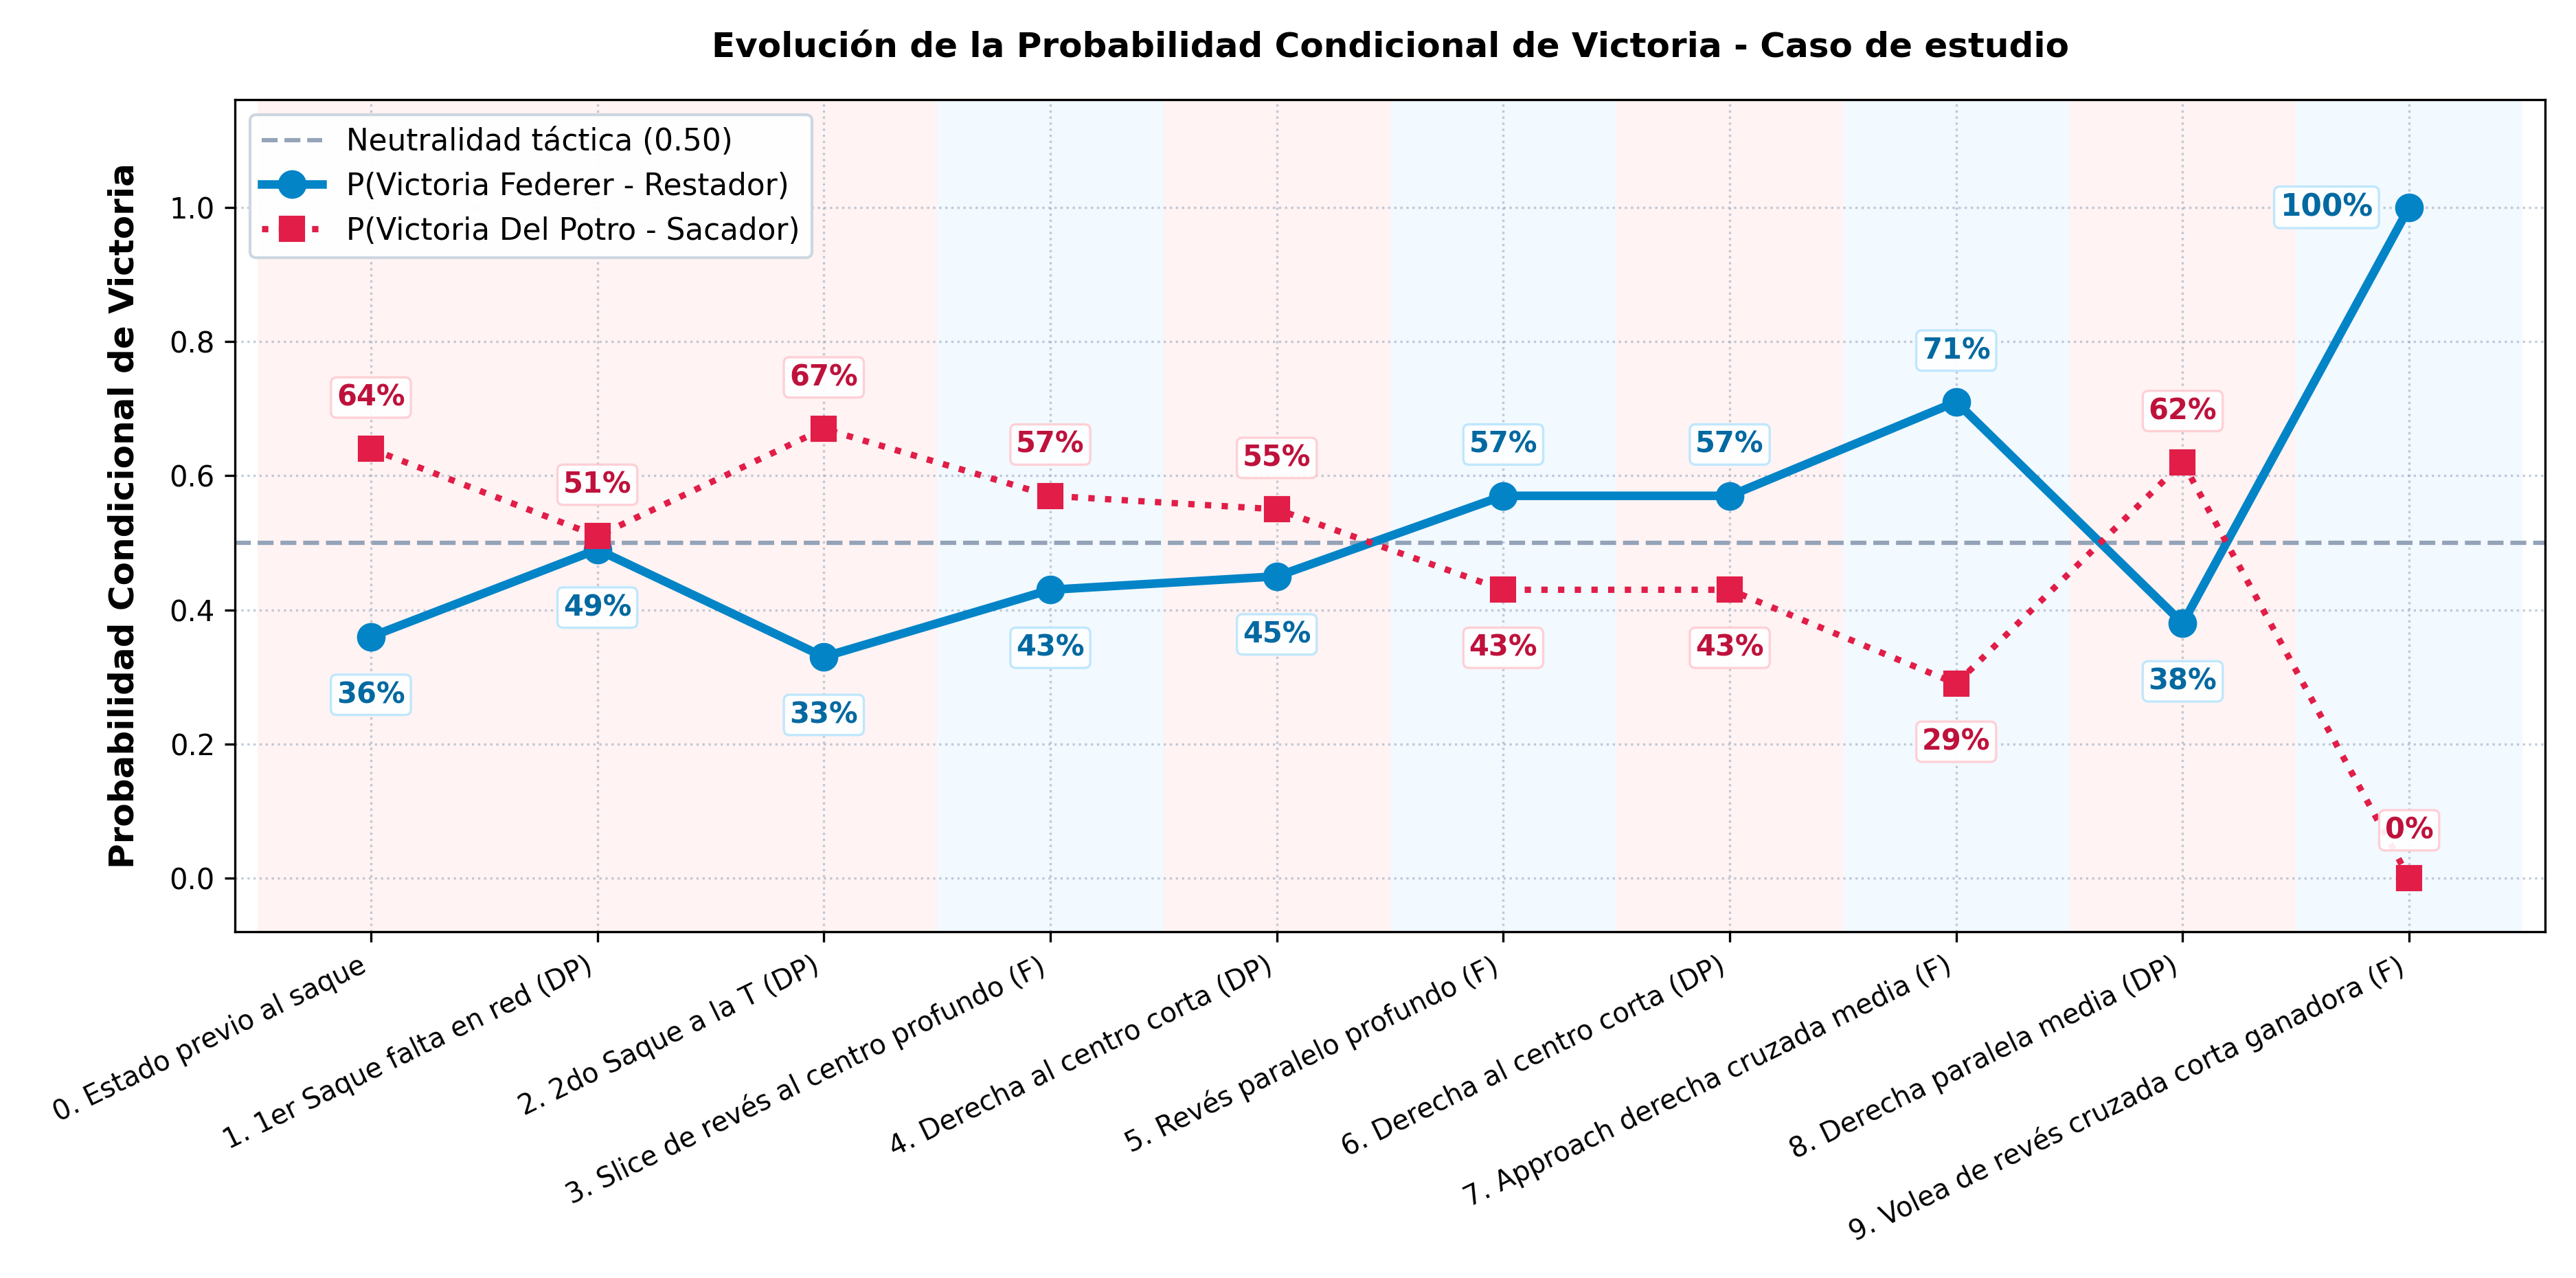
\includegraphics[width=0.95\textwidth]{eval_bar_simulation.png}
    \caption{Evolución de la probabilidad condicional de victoria para el caso de estudio.}
    \label{fig:eval_bar_simulation}
\end{figure*}

\subsection{Caso de estudio sobre la final del US Open 2009}
Para ilustrar la interpretabilidad del modelo, se evaluó el primer punto del segundo game de la final del US Open 2009 (Del Potro al servicio frente a Federer), perteneciente al conjunto de prueba. La Figura \ref{fig:eval_bar_simulation} exhibe la evolución continua de las probabilidades condicionales de victoria estimadas tiro a tiro para ambos jugadores. Las probabilidades previas al peloteo corresponden a las tasas basales observadas en el dataset original ($64.30\%$ cuando el sacador juega con su primer saque y $50.96\%$ cuando juega con el segundo).

El cuarto tiro del punto corresponde a una derecha corta al centro ejecutada por el sacador Juan Martín del Potro. Para evaluarla, \textit{XGBoost} recibe como entrada el vector de 58 características One-Hot que la describe. Al ingresar al primero de los 200 árboles, el tiro comienza en el nodo raíz, que pregunta si dos golpes atrás no existía un golpe registrado (\texttt{anteprev\_golpe\_ninguno}). En el tiro 4 vale 0, porque sí existe el golpe de dos posiciones anteriores en el peloteo continuo (el segundo servicio, tiro 2), por lo que el tiro continúa por la rama del árbol correspondiente al valor 0 hasta atravesar otros siete nodos y llegar al nodo hoja 234, que contiene un leaf weight de $-0{,}022680$. \textit{XGBoost} suma ese peso al \texttt{base\_score} de $= 0{,}56534654$, situando el margen tras este primer paso en $+0{,}240210$ ($55{,}97\%$ de probabilidad), y se avanza sucesivamente a través de los siguientes árboles.

Al atravesar los 200 árboles, la corrección conjunta de todos los estimadores asciende a $-0{,}055300$, alcanzando un logit final de $+0{,}207590$ que luego de pasar por la función sigmoide devuelve finalmente $\approx 0{,}5517$, es decir, un $55{,}17\%$ de probabilidad de victoria para el sacador. El cálculo detallado se resume en el Cuadro \ref{tab:recorrido_tiro4}.

\begin{table}[htbp]
    \centering
    \caption{Cálculo del valor del tiro 4 mediante XGBoost}
    \label{tab:recorrido_tiro4}
    \renewcommand{\arraystretch}{1.25}
    \resizebox{\columnwidth}{!}{%
    \begin{tabular}{|c|l|c|}
        \hline
        \multicolumn{3}{|c|}{\textbf{Árbol 1 (Hoja 234)}} \\ \hline
        \textbf{Decisión} & \textbf{Feature} & \textbf{Rama} \\ \hline
        1 & \texttt{anteprev\_golpe\_ninguno} & 0 \\ \hline
        2 & \texttt{subida\_a\_red} & 0 \\ \hline
        3 & \texttt{prev\_subida\_a\_red} & 0 \\ \hline
        4 & \texttt{anteprev\_subida\_a\_red} & 0 \\ \hline
        5 & \texttt{anteprev\_profundidad\_media} & 0 \\ \hline
        6 & \texttt{prev\_profundidad\_profunda} & 1 \\ \hline
        7 & \texttt{direccion\_indefinida} & 0 \\ \hline
        8 & \texttt{direccion\_centro} & 1 \\ \hline
        \multicolumn{3}{|c|}{\textbf{Predicción del Ensamble}} \\ \hline
        \textbf{Componente} & \textbf{Expresión} & \textbf{Aporte} \\ \hline
        Sesgo base & $b_0 = \ln(p_0 / (1 - p_0))$ & $+0{,}262890$ \\ \hline
        Árbol 1 & $f_1(x)$ (\textit{leaf weight}) & $-0{,}022680$ \\ \hline
        200 árboles & $\sum_{m=1}^{200} f_m(\mathbf{x})$ & $-0{,}055300$ \\ \hline
        Logit final & $z = b_0 + \sum_{m=1}^{200} f_m(\mathbf{x})$ & $+0{,}207590$ \\ \hline
        \textbf{Probabilidad final} & $\sigma(z) = 1 / (1 + e^{-z})$ & \textbf{55,17\%} \\ \hline
    \end{tabular}%
    }
\end{table}

\section{Conclusión}
Este trabajo traslada al tenis profesional el principio de evaluación secuencial utilizado en el ajedrez, definiendo una métrica que estima la probabilidad condicional de victoria del sacador tras cada golpe a partir de los features dinámicos del intercambio. La ventana tripartita contiene señal suficiente para rastrear las fluctuaciones de ventaja del punto con alta velocidad de cómputo. El principal aporte metodológico de este trabajo reside en la ingeniería de características propuesta, que combina el anonimato de los jugadores, la exclusión de variables contextuales estáticas y la ventana temporal tripartita (t, t$-$1, t$-$2).

Sin embargo, el desempeño predictivo obtenido todavía resulta insuficiente para considerar su aplicación directa como instrumento de evaluación táctica durante las transmisiones de tenis profesional. Aun así, los resultados demuestran que es posible extraer información predictiva de la secuencia reciente de golpes sin recurrir a la identidad de los jugadores ni a variables contextuales estáticas.

No obstante, se cita como obstáculo que al carecer de variables cinemáticas continuas como la velocidad, la trayectoria o la posición de los jugadores, múltiples ejecuciones físicamente diferentes colapsan bajo una misma categoría notacional. En trabajos futuros, se podría pensar en incorporar datos de seguimiento óptico continuo para describir la cinemática tridimensional de la pelota y los competidores. Se sugiere también explorar ventanas completas que abarquen todos los golpes previos de la secuencia del punto más allá de la ventana tripartita propuesta.

\bibliographystyle{IEEEtran}
\bibliography{Bibliografia}

\end{document}